\chapter{REVISÃO DA LITERATURA}
\thispagestyle{empty}

\section{Conceitos Básicos}
\subsection{Projetos}

  \citeonline[p. 8]{meredith2011project} definem que projetos tratam da realização de tarefas específicas e finitas, de grande ou pequena escala, com um prazo de execução e um orçamento estipulado. \citeonline{turner2014handbook}, por sua vez, dispõe que projetos são tarefas com uma data final, onde caso esta data não implique na entrega do projeto, será estabelecida uma entrega do produto presente e a criação de outro projeto para entregar as tarefas restantes, referente a este produto.

  Para \citeonline{kerzner2013project} um projeto pode ser caracterizado por uma série de atividades e tarefas realizadas com um objetivo específico para serem completadas sob determinadas especificações. Essas atividades e tarefas também devem possuir datas definida para inicio e fim; limites de recursos e custos; bem como um quantitativo de pessoas e equipamentos que será envolvido nestas.

  Finalmente, de acordo com o \citeonline{pmiguide2014}, um projeto pode ser compreendido por um esforço temporário empreendido a fim de criar um produto, prestar serviço ou trazer um resultado exclusivo. Esse esforço é composto por um conjunto de atividades inter relacionadas e direcionadas à obtenção de um ou mais produtos únicos, com tempo e custos definidos. Nesta definição, algumas características básicas do projeto devem ser destacadas:

  \begin{itemize}
    \item{\textbf{Delimitação temporal:} datas específicas para início e fim;}
    \item{\textbf{Objetivos:} metas definidas em função de um problema, oportunidade ou interesse da organização;}
    \item{\textbf{Elaboração progressiva:} etapas contínuas de desenvolvimento e incrementos;}
    \item{\textbf{Incerteza:} a representação do degrau entre o resultado esperado e as condições de realização do projeto;}
    \item{\textbf{Singularidade:} a representação da exclusividade do projeto, aquilo que o torna único;}
    \item{\textbf{Relação fornecedor-beneficiário:} relação entre quem desenvolve e quem recebe o projeto.}
  \end{itemize}

  Assim, pode-se compreender que todo projeto é essencialmente temporário e único, ou ainda, finito e regular, que frequentemente é utilizado, direta ou indiretamente, para alcançar os objetivos de um plano estratégico que, por sua vez, visa o desenvolvimento de um novo produto ou um serviço exclusivo.

\subsection{Gestão de Projetos}

  De acordo com \citeonline[p. 74]{kerzner2013project} a gestão de projetos pode ser considerada uma metodologia que consiste em um processo repetitivo usado em projetos com o objetivo de alcançar sua maturidade. Afirma-se também que qualquer metodologia, inclusive a mais simples, pode representar um caso de sucesso como prática de GP, desde que seja aceita na organização em questão. Entretanto, ao utilizar uma metodologia de GP de sucesso, a probabilidade de que a organização se destaque como entregadora de bons projetos será elevada \cite{kerzner2013project}.

  Para \citeonline{pmiguide2014}, a GP implica no uso de ferramentas, técnicas e da competência de utilizar recursos como: o conhecimento de conceitos, características próprias e particulares, bem como fatores críticos de sucesso para o aprimoramento e entrega de projetos de excelência. O guia PMBOK é considerado um conjunto das melhores práticas de GP, que se encontra dividida em cinco grupos de processos e dez áreas de conhecimento \cite{pmiguide2014}.

  São os grupos de processos:
  \singlespacing
  \begin{enumerate}
    \item Iniciação;
    \item Planejamento;
    \item Execução;
    \item Monitoramento e Controle;
    \item Encerramento.
  \end{enumerate}
  \onehalfspacing

  Quanto as áreas de conhecimento, constam os gerenciamentos de:

  \singlespacing
  \begin{enumerate}
    \item Integração;
    \item Escopo;
    \item Tempo;
    \item Custos;
    \item Qualidade;
    \item Recursos Humanos;
    \item Riscos;
    \item Comunicação;
    \item Aquisições;
    \item Partes Interessadas.
  \end{enumerate}
  \onehalfspacing


  A Figura~\ref{processos_areas_pmbok} representa a divisão da relação das àreas de conhecimento pelos grupos de processos.

  \begin{figure}[ht]
    \centering
    \scalebox{0.3}{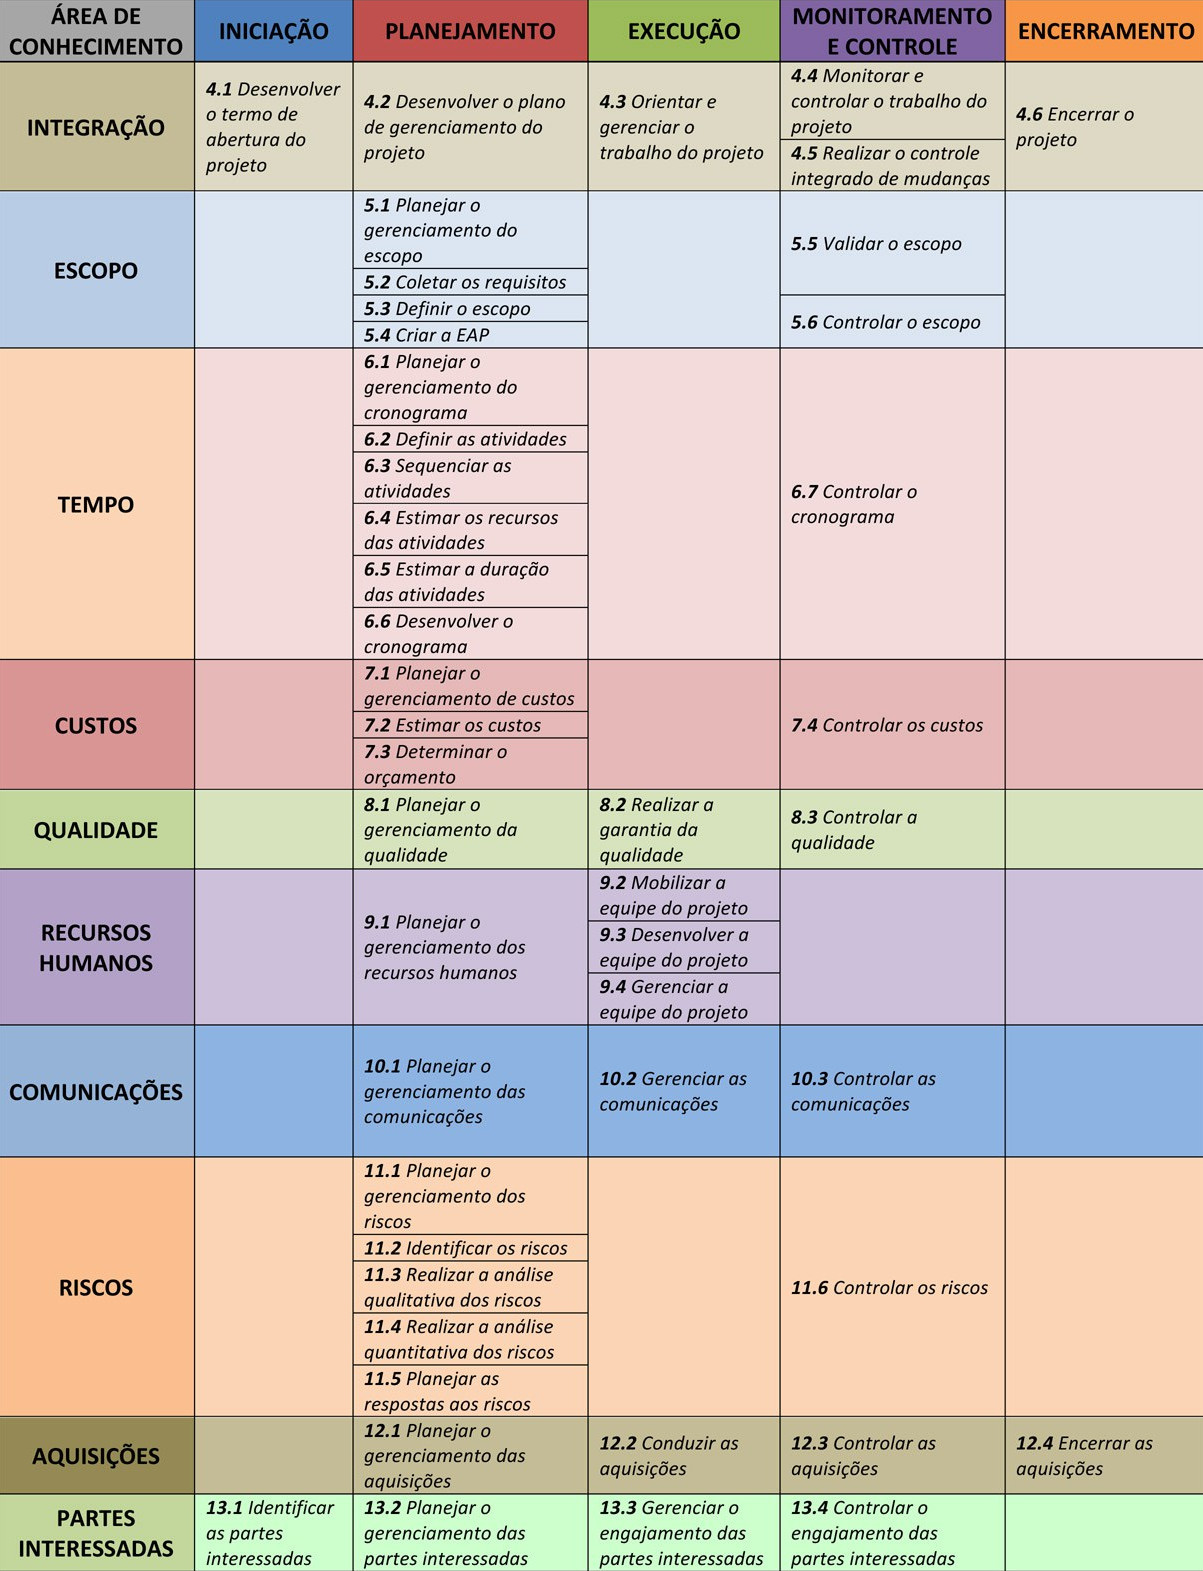
\includegraphics{figuras/processos_areas_pmbok}}
    \caption{Relação dos grupos de processos pelas àreas de conhecimento. Fonte: \cite{pmiguide2014}}
    \label{processos_areas_pmbok}
  \end{figure}

  Alguns autores afirmam que a garantia de que os objetivos definidos de projeto serão alcançados depende de um processo disciplinado, por parte da GP, que respeite custos, prazos e desempenho requeridos e que ocorra através do envolvimento de pessoas em atividades de planejamento e controle numa organização \cite{dinsmore2009ama, meredith2011project}.

\subsection{Gestão de Programas}

  Programas podem ser entendidos por estruturas que consistem em uma equipe principal e um conjunto de equipes de projeto que averiguam capacidade de decisão e autoridade de um membro definitivo, isto é, um gerente de programa que assegura a direção e as decisões desta estrutura. Estas estruturas visam alcançar um determinado objetivo dentro de uma estratégia.\cite{brown2008handbook}.

  \citeonline{rijke20141197} avalia que apesar da dificuldade geral em distinguir um programa de um projeto, a gestão de programas deve ser considerada mais extensa que gestão de projetos, pois ela abrange áreas em que projetos singulares não se encontram. Vale ressaltar também que o gestor de programa tem hábitos mais estratégicos que podem interferir na GP \cite{lycett2004289}.

  Assim, a gestão de programas tem sido cada vez mais adotada por organizações com o objetivo de implementar estratégias que integrem melhor seus projetos e ferramentas, sem permitir que o desempenho possa desorientar a natureza estratégica das decisões.

\subsection{Gestão de Portfólio}

  A gestão de portfólio, conhecida também por Gestão de Portfólio de Projetos (GPP), surgiu a partir da necessidade de gerenciar investimentos em projetos nas organizações. Seu processo dinâmico e integrado visa avaliar o alinhamento estratégico e a viabilidade da execução simultânea de diversos projetos ao mesmo tempo. Esses projetos passam por uma introspecção que os seleciona e organiza de acordo com sua priorização em um portfólio \cite{meredith2011project, kerzner2013project}.

  De acordo com \citeonline[p. 27]{burke2013project}, um portfólio pode abrigar conjuntos de projetos, programas e até mesmo outros portfólios que não precisam estar diretamente relacionados, mas que se reúnem por uma questão de otimização e controle. A Figura~\ref{port_prog_proj} ilustra a relação entre portfólio, programas e projetos.

  \begin{figure}[ht]
    \centering
    \scalebox{0.4}{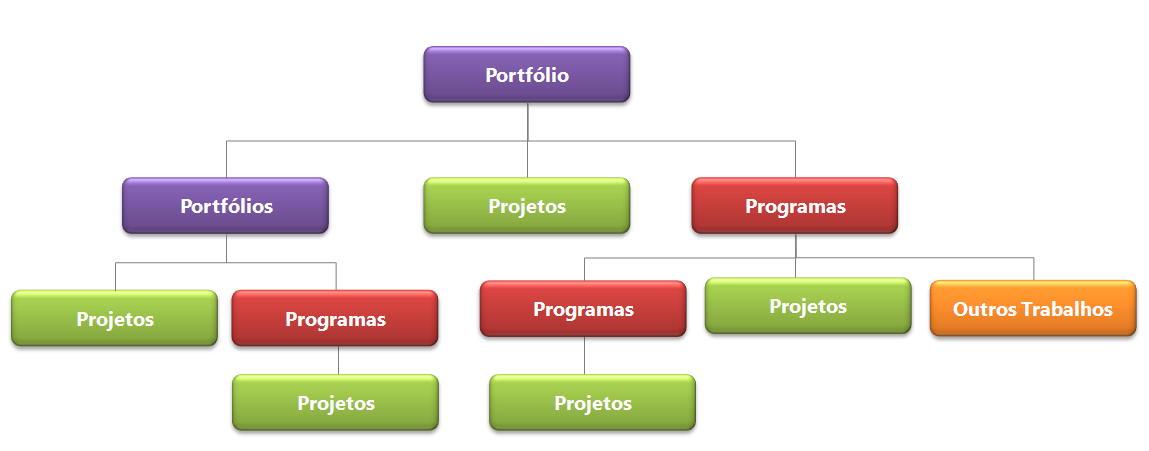
\includegraphics{figuras/port-prog-proj}}
    \caption{Relação Portfólio, Programas e Projetos. Fonte: \cite{pmi2006}}
    \label{port_prog_proj}
  \end{figure}

  \citeonline[p 11]{pmiguide2014} estabelece que o critério de agrupamento de um portfólio deve visar a facilitação na gestão para que seja possível atingir os objetivos estratégicos de uma organização. É definido ainda que toda gestão de portfólio fique sob responsabilidade de um EGP. A figura \ref{estrategia_portfolio} representa os processos incorporados pela Gestão de Portfólio.

  \begin{figure}[ht]
    \centering
    \scalebox{0.4}{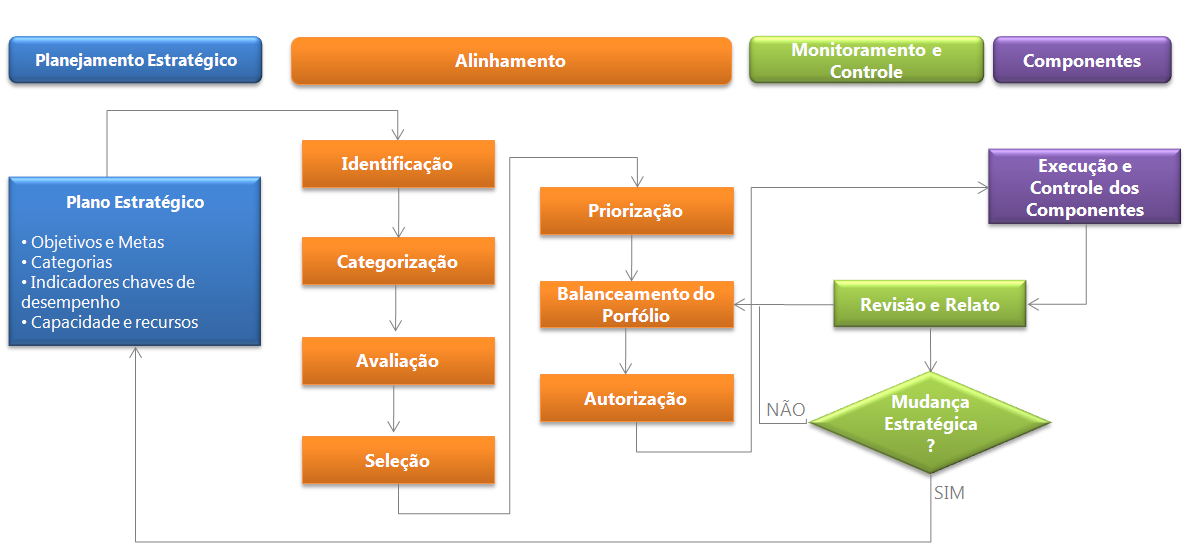
\includegraphics{figuras/estrategia-portfolio}}
    \caption{Processos de Gestão de Portfólio. Fonte: \cite{pmi2006}}
    \label{estrategia_portfolio}
  \end{figure}

  Desta forma, a GPP pode ser dita como uma manifestação de estratégia de negócios que determina os investimentos da organização via processos simultâneos, sistemáticos e dinâmicos de decisão, tornando o sucesso do EGP dependente do desempenho agregado de iniciativas dos componentes do portfólio e buscando a maximização do uso e do alinhamento desses componentes \cite{pmiguide2014}.

\subsection{Escritorio de Gestão de Projetos}

  Advindo do inglês \textit{Project Management Office}(PMO), o escritório de gestão de projetos (EGP), ou ainda escritório de projetos (EP), pode ser considerado um conjunto de profissionais de GP que servem a um modelo organizacional com o propósito de aumentar a eficiência e lidar com as necessidades da GP, assumindo um papel de alta confiança ao implementar diversas estratégias em projetos \cite{kendall2003advanced}.

  Através de um estudo, \citeonline{pemsel2013project} identificou três principais atividades que são esperadas do EGP:

  \begin{itemize}
    \item Promover e facilitar o desenvolvimento estratégico da GP, bem como o uso estratégico de objetos que sejam empreendidos na GP;
    \item Planejar, controlar e dar suporte a GP, sempre assegurando que o conhecimento seja compartilhado no processo para melhorar sua eficiência;
    \item Adoção estratégias de treinamento, negociação e formação para prover o desenvolvimento de competências.
  \end{itemize}

  Para \citeonline{dinsmore2005pmo} a principal expectativa empregada por um EGP esta relacionada ao suporte e orientação; ao processo de desenvolvimento e gerenciamento de projetos mais eficiente e eficaz o possível; e ao uso de metodologias e recursos de planejamento e análise de projetos padronizadas.

  De acordo com \citeonline{crawford2010strategic}, por mais simples que um EGP possa ser, suas atividades compõem estruturas complexas responsáveis por atividades de planejamento, controle e monitoramento, cuja implantação representa um processo de mudança de cultura organizacional, por estar diretamente relacionada à negociação com pessoas. O autor retrata ainda três níveis de atuação do EGP que podem ser visualizados na Figura~\ref{pmo_crawford}.

  \begin{figure}[ht]
    \centering
    \scalebox{0.6}{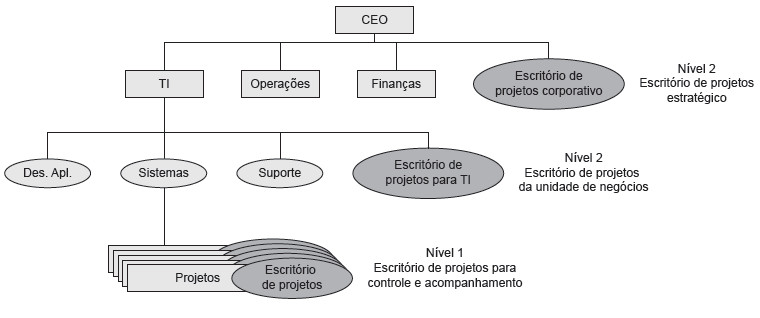
\includegraphics{figuras/pmo-crawford}}
    \caption{Níveis de atuação do escritório de projetos. Fonte: \cite{crawford2010strategic}.}
    \label{pmo_crawford}
  \end{figure}

  As competências desses níveis podem ser representas como \cite{crawford2010strategic}:

  \begin{itemize}
    \item \textbf{Nível 1 - Escritório de Controle de Projetos:} visa o desenvolvimento do planejamento de projetos individualmente, realizando também a emissão de relatórios de progresso. Embora tenha foco em apenas um projeto, geralmente este projetos apresenta grande porte e complexidade;
    \item \textbf{Nível 2 - Escritório de Projetos da Unidade de Negócios:} oferece suporte a todos os projetos de uma área específica, porém de porte e complexidade variados;
    \item \textbf{Nível 3 - Escritório Estratégico de Projetos:} possui as seguintes competências:
    \begin{itemize}
      \item Selecionar, priorizar e garantir a integração de cada projeto para que esteja alinhado à estratégia da organização, inclusive no que respeito aos seus recursos;
      \item Desenvolver, atualizar e divulgar a metodologia de GP bem como seus conhecimentos;
      \item Converte-se em centro da gestão de conhecimento da organização através do armazenamento de informações sobre lições aprendidas;
      \item Validar estimativas de recursos realizadas pelo projetos, baseando-se em experiências anteriores.
    \end{itemize}
  \end{itemize}

  Assim, as responsabilidades de um EGP podem variar de acordo com a centralização empregada na organização, uma vez que está relacionada a padronização dos processos de GP. Entretanto as ferramentas e técnicas a serem empregadas ficam sob critério do gestor responsável pelo EGP \cite{pmiguide2014}.

  Alguns autores, ainda, apontam o EGP como uma ferramenta de apoio para que organizações obtenham bom desempenho em GP, bom como para alcançarem seus objetivos estratégicos. Esses mesmos autores destacam que fatores comuns ligados as taxas de sucesso do EGP, em caso positivo, devem ser enfatizados, enquanto em caso negativos, devem ser evitados, configurando assim boas práticas para o sucesso do EGP \cite{andersen2007benchmarking}.

\subsection{Sistemas de Gestão de Projeto}

  Ao contrário do que é esperado pela natureza de negócios ou operações usuais, a natureza dos projetos e serviços é representada por processos curtos, repetitivos e funcionais, que facilitam a identificação de padrões usualmente inseridos em soluções de informação. Assim, especialista de GP veem o uso de sistemas de gestão de produtos (SGP), como uma ferramenta preciosa no que respeito a alcanço os objetivos e na excelência de projetos \cite{cserban2011project}.

  Seguindo mais além, \citeonline{prado2006mmgp} afirma que diversos aspectos das metologias de GP dependem indiretamente do uso de SGP, sem que porém, seja determinada a natureza do SGP. O autor infere ainda que só é possível para organizações almejarem determinados níveis de maturidade se utilizarem essas ferramentas.

  Através de um estudo quantitativo, \citeonline{liberatore2001project} analisou que nunca antes a adoção de uma ferramenta para auxiliar nas práticas de GP foi tão explorada quanto o uso de SGP. Os especialistas de GP demonstraram grande interesse pela facilidade encontrada no compreendimento da complexidade do projeto através desses sistemas, e expressaram interesse em integrar cada vez funcionalidades referente aos projetos.

  Por meio de uma revisão na literatura \citeonline{hartmann2009implementing}, acrescentou que além de auxiliar no tratamento da complexidade nos projetos, o uso de SGP também se destaca para o aprimoramento da produtividade do processo de projeto, apesar de também ser notada uma dificuldade inicial para o adaptamento do uso dessas ferramentas.

  Além de prover um meio para lidar com a produtividade de processo e complexidade do projeto, já foi comprovado também que o uso de SGP influi nos processos de planejamento, comunicação, monitoramento, controle de riscos, cronograma, gerenciamento de documentos e ainda avaliação de custos \cite{raymond2008project}.

  Portanto, o uso de SGP implica em deter ferramentas capazes de facilitar e otimizar o esforço empregado pela GP para alcançar a excelência na realização do projeto, não apenas por parte do uso dos gestores do projeto, mas também por incluir outros atores presentes em seus processos \cite{cserban2011project}.

\section{Associações de Gestão de Projetos}

  \begin{quadro}[!htpb]
    \centering
    \label{quadro-institutos}
    \caption{Principais associações de Gestão de Projetos \\ Fonte: Adaptação de \citeonline{patah2012metodos}}
    \begin{tabular}{| m{.40\textwidth} m{.30\textwidth} m{.20\textwidth}|}
      \hline
      \textbf{Institutos} & \textbf{Conjunto de Métodos} & \textbf{País de Origem} \\
      \hline \hline
      \textit{Project Management Institute} (PMI) & \textit{Project Management Body of Knowledge} (PMBoK) & EUA \\ \hline
      \textit{International Project Management Association} (IPMA) & IPMA \textit{Competence Baseline} & União Européia \\ \hline
      \textit{Association for Project Management} (APM) & APM \textit{Body of Knowledge} & Reino Unido \\ \hline
    \end{tabular}
  \end{quadro}

  \subsection{Project Management Institute (PMI)}

  O PMI foi fundado em 1969, como uma instituição sem fins lucrativos, que se baseou na premissa de que existiam muitas práticas comuns de GP em diversas áreas de projetos, entre elas, nas áreas de contrução e de produção farmaceútica (PMI, 2008; PMI, 2010a). Atualmente esse instituto é conhecido por disseminar o conhecimento sobre GP em diversos paises, sendo sua sede situada nos Estados Unidos (EUA), conforme ilustrado no Quadro~\ref{quadro-institutos}

O PMI foi fundado em 1969, é um dos institutos que atua no desenvolvimento e disseminação do conhecimento de Gestão de Projetos. Sua sede é nos Estados Unidos, e possui 240.000 membros distribuídos em mais de 160 países. Suas certificações e publicações são reconhecidas mundialmente, entre elas o PMBOK - Project Managemant Body of Knowledge. O PMI possui representações locais chamadas capítulos 1 . Prado e Archibald (2004, p. 17) afirmam que o PMI é quem padroniza e comanda a maioria das ações deste assunto em todo o mundo”.

De modo geral, o que se observa é que o PMBoK é um conjunto de métodos genérico e bastante abrangente que objetiva atender às necessidades dos mais diversos tipos de projetos (PMI, 2008).
O PMI (2009) apresenta um número de US\$ 12 trilhões, um quinto do valor do PIB mundial, como o valor a ser investido em projetos em cada um dos anos da atual década.

296.377 é o número de filiados ao PMI;11
o número de filiados cresceu 13,8\% entre fevereiro de 2008 e fevereiro de 2009;
existem 327.250 gerentes de projetos certificados PMP no mundo;
existem 7.207 profissionais certificados Certified Associate in Project Management (CAPM) no mundo;
o número de visitas (feitas apenas em janeiro e fevereiro deste ano) à website
oficial do PMI é de 2.444.645.

Conforme o PMI (2010a), ao longo de sua existência, o Instituto desenvolveu ferramentas que auxiliam o desenvolvimento de esforços de projetos. Uma dessas ferramentas, ou meios, de atualização é o complexo criado e mantido pelo mesmo, formado por publicações periódicas (PM Today, PM Journal, PM Network), publicações de padrões normativos (Project Management Body of Knowledge, The Standar for Portfólio Management, The Standar for Program Management, Government Extension for PMBOK Guide, Contruction Extension for PMBOK, entre outros), website, eventos regionais e globais (Global Congresses) e certificações (CAPM, PMP, PMI-SP, PgMP, PMI-RMP).
Aborda, como destacado em seu título para a publicação em português, “Um Guia do Conjunto de Conhecimentos em Gerenciamento de Projetos”, e é considerado bibliografia indispensável para o Gerenciamento de Projetos e para a Certificação PMP.

Da mesma forma, esse projeto trazia, como sugestão para desenvolvimento, as mesmas três áreas de concentração (ética, normas e credenciamento) (PMI, 2008). São elas:
y as características distintas de um profissional (ética);
y o conteúdo e a estrutura do conjunto de conhecimentos da profissão (normas);
y o reconhecimento de capacitação profissional (credenciamento).

Nesse projeto, o conteúdo original foi ampliado e reestruturado, agregando mais três
novas seções. São elas:
y inclusão da estrutura de Gerenciamento de Projetos para cobrir as relações entre o projeto e o seu ambiente externo, e também entre o Gerenciamento de Projetos e o gerenciamento geral;
y inclusão do gerenciamento de riscos como mais uma Área de Conhecimento;
y inclusão do gerenciamento de contratos/aquisições como mais uma Área de
Conhecimento.
Finalizando o ciclo com diversas mudanças e correções editoriais, em março de
1987, a Diretoria do PMI aprovou o manuscrito final como um documento
independente. Esse manuscrito foi publicado no mesmo ano com o nome Project
Management Body of Knowledge ou “O Conjunto de Conhecimento em
Gerenciamento de Projetos” (PMI, 2008).

O Guia PMBOK 5a edição, padrão do PMI para Gestão de Projetos, apresenta como melhores práticas, 47 processos de gerenciamento de projetos, distribuídos em 5 grupos de processos. Conforme o anexo 1, são eles: [1] iniciação, [2] planejamento, [3] execução, [ 4] monitoramento e controle e [5] encerramento. (PMI, 2013, p. 5).


  \subsection{International Project Management Association (IPMA)}

  \subsection{Association for Project Management (APM)}


\section{Maturidade em Gestão de Projetos}

Maturidade é o desenvolvimento de sistemas e processos que são por
natureza repetitivos e garantem uma alta probabilidade de que cada
um deles seja um sucesso. Entretanto, processos e sistemas repetitivos
não são, por si só, garantia de sucesso. Apenas aumentam a sua
probabilidade. Harold Kerzner

A maturidade é uma qualidade ou estado de amadurecimento. Se
aplicarmos o conceito de maturidade em uma organização, podemos relacionar a
maturidade com o estado no qual a organização está em perfeitas condições para
alcançar seus objetivos

Atualmente as organizações são avaliadas quanto ao nível de maturidade
dentro de uma escala definida por cada um dos modelos de maturidade em gestão de
projetos já propostos.

Os modelos de maturidade partem da premissa que as organizações,
pessoas e setores evoluem por meio de um processo contínuo de desenvolvimento ou
crescimento em direção a uma maturidade mais avançada. Os modelos têm por
finalidade auxiliar na elaboração de processos e execução de melhores práticas para
que as organizações se desenvolvam de forma constante.

> maturidade em gestao de projetos

Maturidade em Gestão de Projetos, ou maturidade organizacional em Gestão de Projetos é definido pelo PMI (2013, p. 552) como “o nível de habilidade de uma organização de entregar os resultados estratégicos desejados de maneira previsível, controlável e confiável”.
Em outras palavras, a maturidade em GP pode ser entendida como a nível de habilidade e conhecimento da organização para gerenciar seus projetos e obter sucesso, considerando que o sucesso está relacionado com a conclusão do projeto dentro do escopo, prazo, custo e qualidade planejado, satisfação do cliente, entre outros aspectos.
Kerzner (2000, apud RABECHINI JR., p. 33) apresenta um ciclo de vida da Gestão de Projetos, conforme a Figura~\ref{ciclo-maturidade}.

  \begin{figure}[ht]
    \centering
    \scalebox{0.6}{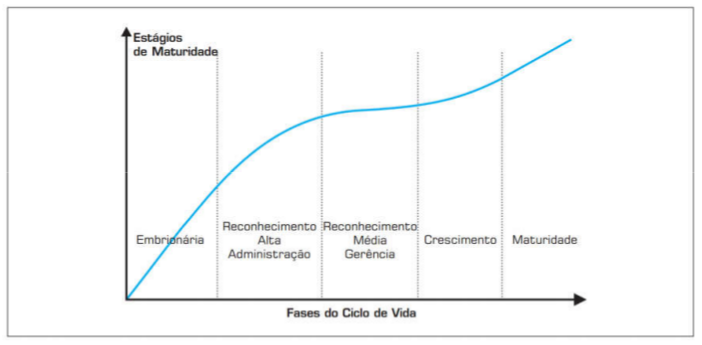
\includegraphics{figuras/ciclo-maturidade}}
    \caption{Ciclo de Vida da Gestão de Projetos.\\ Fonte: Adaptado de \cite{kerzner2006projeto}.}
    \label{ciclo-maturidade}
  \end{figure}

Os modelos de maturidade mais utilizados no Brasil são o OPM3 – Organizational Project Management Maturity Model, proposto pelo PMI, e o MMGP – Modelo de Maturidade em Gerenciamento de Projetos, proposto por Prado e Archibald. Conforme o PMSURVEY 10 do PMI (2014b, p. 42), este último é o modelo de maturidade mais utilizado entre nas instituições públicas brasileiras.

Os principais modelos existentes apresentam cinco níveis de maturidade, mas diferem um pouco quanto ao conteúdo de cada nível.
Prado e Archibald (2015) afirmam que quanto maior a maturidade, [1] maior o índice de sucesso total, [2] menor o índice médio de atraso, [3] menor o estouro médio de custos e [4] maior a confiança da alta administração em sua capacidade de planejar e executar projetos com sucesso.


> PMMM
> CMM-I???
> OPM3
  \subsubsection{Modelo de Maturidade em Gerenciamento de Projetos}

    \begin{figure}[ht]
      \centering
      \scalebox{0.6}{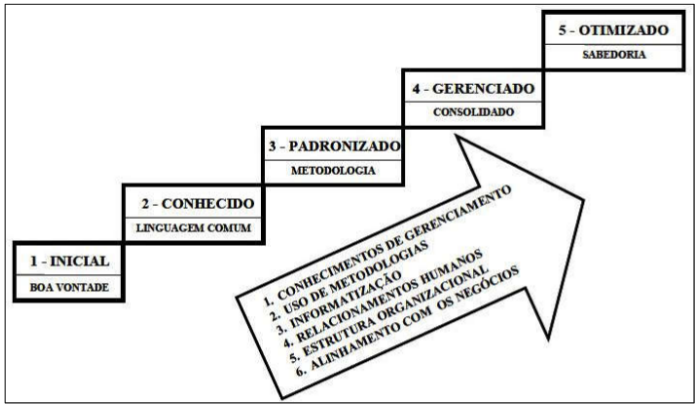
\includegraphics{figuras/mmgp}}
      \caption{Dimensões e níveis de maturidade do modelo Prado - MMGP.\\ Fonte: Prado e Archibald (2006, p.131).??? \cite{kerzner2006projeto}.}
      \label{mmgp}
    \end{figure}

\section{Fatores Críticos de Sucesso}
> conceito sucesso
Sucesso em Gestão de Projetos é frequentemente definido como a conclusão do projeto com atendimento da totalidade do escopo dentro do prazo e custo planejados e com a qualidade esperada. No entanto, existem variações deste entendimento.
Shenhar, Levy e Dvir (1997 apud NORO; BONZATTI, 2013, p. 86) afirmam que as pessoas possuem diferentes percepções em relação ao conceito de sucesso, e que essa percepção varia no tempo.
Kerzner (2006, p. 41-42) afirma que “o problema de definir sucesso como a concretização do prazo programado, dentro do orçamento e com níveis de qualidade desejado é que todos estes indicadores constituem uma definição interna de sucesso”. Segundo o autor o sucesso é definido pelo cliente. “Pode-se concluir um projeto internamente no prazo, no orçamento e nos limites de qualidade para só então descobrir que o cliente não gostou dos resultados.”

Vargas (2003, p. 18) afirma que “um projeto bem-sucedido é aquele que é realizado conforme planejado”. Como a maioria dos autores, Vargas (2003, p. 19) considera que o sucesso de um projeto pode ser medido pela obtenção dos resultados esperados, dentro do prazo, custo e qualidade desejados. Porém, ressalta que outros parâmetros são importantes. O autor define os seguintes critérios para considerar um projeto como bem-sucedido:
- Ser concluído dentro do tempo previsto;
- Ser concluído dentro do orçamento previsto;
- Ter utilizado recursos (materiais, equipamentos e pessoas) eficientemente, sem desperdícios;
- Ter atingido a qualidade e a performance desejada;
- Ter sido concluído com o mínimo possível de alteração de seu escopo;
- Ter sido aceito sem restrições pelo contratante ou cliente;
- Ter sido empreendido sem que ocorresse interrupção ou prejuízo nas atividades normais da organização;
- Não ter agredido a cultura da organização.

Prado e Archibald (2015) classificam os projetos em três categorias quanto ao sucesso:
Sucesso total: Um projeto bem-sucedido é aquele que atingiu a meta. Isto geralmente significa que foi concluído e produziu os resultados e benefícios esperados e os principais envolvidos ficaram plenamente satisfeitos. Além disso, mas não obrigatoriamente, espera-se que o projeto tenha sido encerrado dentro das exigências previstas para prazo, custo, escopo e qualidade (pequenas diferenças podem ser aceitas).
Sucesso parcial ou comprometido: o projeto foi concluído, mas não produziu todos os resultados e benefícios esperados. Existe uma significativa insatisfação entre os principais envolvidos. Além disso, provavelmente algumas das exigências previstas para prazo, custo, escopo e qualidade foram significativamente excedidas.
Fracasso: existe uma enorme insatisfação entre os principais envolvidos ou porque o projeto não foi concluído ou porque não atendeu às expectativas dos principais envolvidos ou porque algumas das exigências previstas para prazo, custo, escopo e qualidade foram excedidas de forma absolutamente inaceitável.

Conforme o PMI (2015, p. 8) a pesquisa Pulse revelou em média o percentual de projetos bem sucedidos é de 64\%, sendo considerado como projeto bem-sucedido aquele que atinge seus objetivos. O PMI (2015, p. 5) acredita que até que mais organizações comecem a investir na compreensão do valor da GP, no desenvolvimento de talentos (capacitação) na padronização de processos, as taxas gerais de sucesso de projetos não irão melhorar.

> fatores críticos de sucesso em GP

